\documentclass[fleqn]{hermans-hw}

%\usepackage{haldefs}
\usepackage{amsmath}
\usepackage{float}
\usepackage{notes}
\usepackage{url}
\usepackage{graphicx}
\title{HW1: Search}
\duedate{}
\class{CS6300: Artificial Intelligence, Spring 2018}
\institute{University of Utah}
\author{Jake Pitkin}
% IF YOU'RE USING THIS .TEX FILE AS A TEMPLATE, PLEASE REPLACE
% The author WITH YOUR NAME AND UID.
% Replace the due date with anyone you worked with i.e. "Worked with: John McCarthy, Watson, & Hal-9000"

\begin{document}

\maketitle
\section{Graph Search}

For the following problems, S will denote Start and G will denote Goal. When choosing an arbitrary order of state expansions, alphabetical ordering will be used. Once visited, a state will not be expanded again.

\begin{enumerate}
\item Greedy search

\begin{table}[H]
\centering
{\renewcommand{\arraystretch}{1.2}%
\begin{tabular}{| c | c | c |}
\hline
\textbf{Step} & \textbf{Frontier} & \textbf{Expand}\\
\hline
1 & (S, 0) & S\\ \hline
2 & (S-A, 3), (S-B, 2) & B\\ \hline
3 & (S-A, 3), (S-B-D, 1), (S-B-C, 2), (S-B-G, 4) & D\\ \hline
4 & (S-A, 3), (S-B-C, 2), (S-B-G, 4), (S-B-D-G, 5) & C\\ \hline
5 & (S-A, 3), (S-B-G, 4), (S-B-D-G, 5), (S-B-C-G, 1) & G\\ \hline
\end{tabular}}
\caption{Greedy search}
\end{table}

\textbf{Greedy search final path: $S \rightarrow B \rightarrow C \rightarrow G$}

\item Depth first search
 
Note: as a LIFO queue is used, nodes are enqueued in reverse alphabetical order, so they are expanded in alphabetical order.

\begin{table}[H]
\centering
{\renewcommand{\arraystretch}{1.2}%
\begin{tabular}{| c | c | c |}
\hline
\textbf{Step} & \textbf{Frontier} & \textbf{Expand}\\
\hline
1 & S & S\\ \hline
2 & A, B & A\\ \hline
3 & G, B & G\\ \hline
\end{tabular}}
\caption{Depth first search}
\end{table}

\textbf{Depth first search final path: $S \rightarrow A \rightarrow G$}

\item Breadth first search

Note: when adding nodes to the frontier, a check is first made to see if they are already contained in the frontier. If they are, they aren't re-added.

\begin{table}[H]
\centering
{\renewcommand{\arraystretch}{1.2}%
\begin{tabular}{| c | c | c |}
\hline
\textbf{Step} & \textbf{Frontier} & \textbf{Expand}\\
\hline
1 & S & S\\ \hline
2 & A, B & A\\ \hline
3 & B, G & B\\ \hline
4 & G, C, D & G\\ \hline
\end{tabular}}
\caption{Breadth first search}
\end{table}

\textbf{Breadth first search final path: $S \rightarrow A \rightarrow G$}

\item Uniform cost search

\begin{table}[H]
\centering
{\renewcommand{\arraystretch}{1.2}%
\begin{tabular}{| c | c | c |}
\hline
\textbf{Step} & \textbf{Frontier} & \textbf{Expand}\\
\hline
1 & (S, 0) & S\\ \hline
2 & (S-A, 3), (S-B, 2) & B\\ \hline
3 & (S-A, 3), (S-B-C, 4), (S-B-D, 3), (S-B-G, 6) & A\\ \hline
4 & (S-B-C, 4), (S-B-D, 3), (S-B-G, 6), (S-A-G, 6) & D\\ \hline
5 & (S-B-C, 4), (S-B-G, 6), (S-A-G, 6), (S-B-D-G, 8) & C\\ \hline
6 & (S-B-G, 6), (S-A-G, 6), (S-B-D-G, 8), (S-B-C-G, 5) & G\\ \hline
\end{tabular}}
\caption{Uniform cost search}
\end{table}

\textbf{Uniform cost search final path: $S \rightarrow B \rightarrow C \rightarrow G$}

\item Greedy search with the heuristic values listed at each state

\begin{table}[H]
\centering
{\renewcommand{\arraystretch}{1.2}%
\begin{tabular}{| c | c | c |}
\hline
\textbf{Step} & \textbf{Frontier} & \textbf{Expand}\\
\hline
1 & (S, 0) & S\\ \hline
2 & (S-A, 2), (S-B, 3) & A\\ \hline
3 & (S-B, 3), (S-A-G, 0) & G\\ \hline
\end{tabular}}
\caption{Greedy search with heuristic values}
\end{table}

\textbf{Greedy search with heuristic final path: $S \rightarrow A \rightarrow G$}

\item A* search with the heuristic values listed at each state

\begin{table}[H]
\centering
{\renewcommand{\arraystretch}{1.2}%
\begin{tabular}{| c | c | c |}
\hline
\textbf{Step} & \textbf{Frontier} & \textbf{Expand}\\
\hline
1 & (S, 0) & S\\ \hline
2 & (S-A, 5), (S-B, 5) & A\\ \hline
3 & (S-B, 5), (S-A-G, 6) & B\\ \hline
4 & (S-A-G, 6), (S-B-C, 5), (S-B-D, 4), (S-B-G, 6) & D\\ \hline
5 & (S-A-G, 6), (S-B-C, 5), (S-B-G, 6), (S-B-D-G, 8) & C\\ \hline
6 & (S-A-G, 6), (S-B-G, 6), (S-B-D-G, 8), (S-B-C-G, 5) & G\\ \hline
\end{tabular}}
\caption{A* search}
\end{table}

\textbf{A* search final path: $S \rightarrow B \rightarrow C \rightarrow G$}

\end{enumerate}

\newpage
\section{Downhill Skiing}

After getting to Alta, Alice takes the lift up to the top of the
mountain.  The run is really rocky, so her only option is to go
straight downhill.  She begins with a velocity of $0$ and can safely
maintain a maximum velocity of $V$.  At any state, she has three
actions she can take: accelerate, decelerate or coast.  If the
accelerates, her velocity increases by $1$; if she decelerates, it
decreases by $1$; if she coasts, it stays the same.  \emph{After} her
velocity is adjusted by her action, she moves downhill an equal number
of squares to her current velocity.

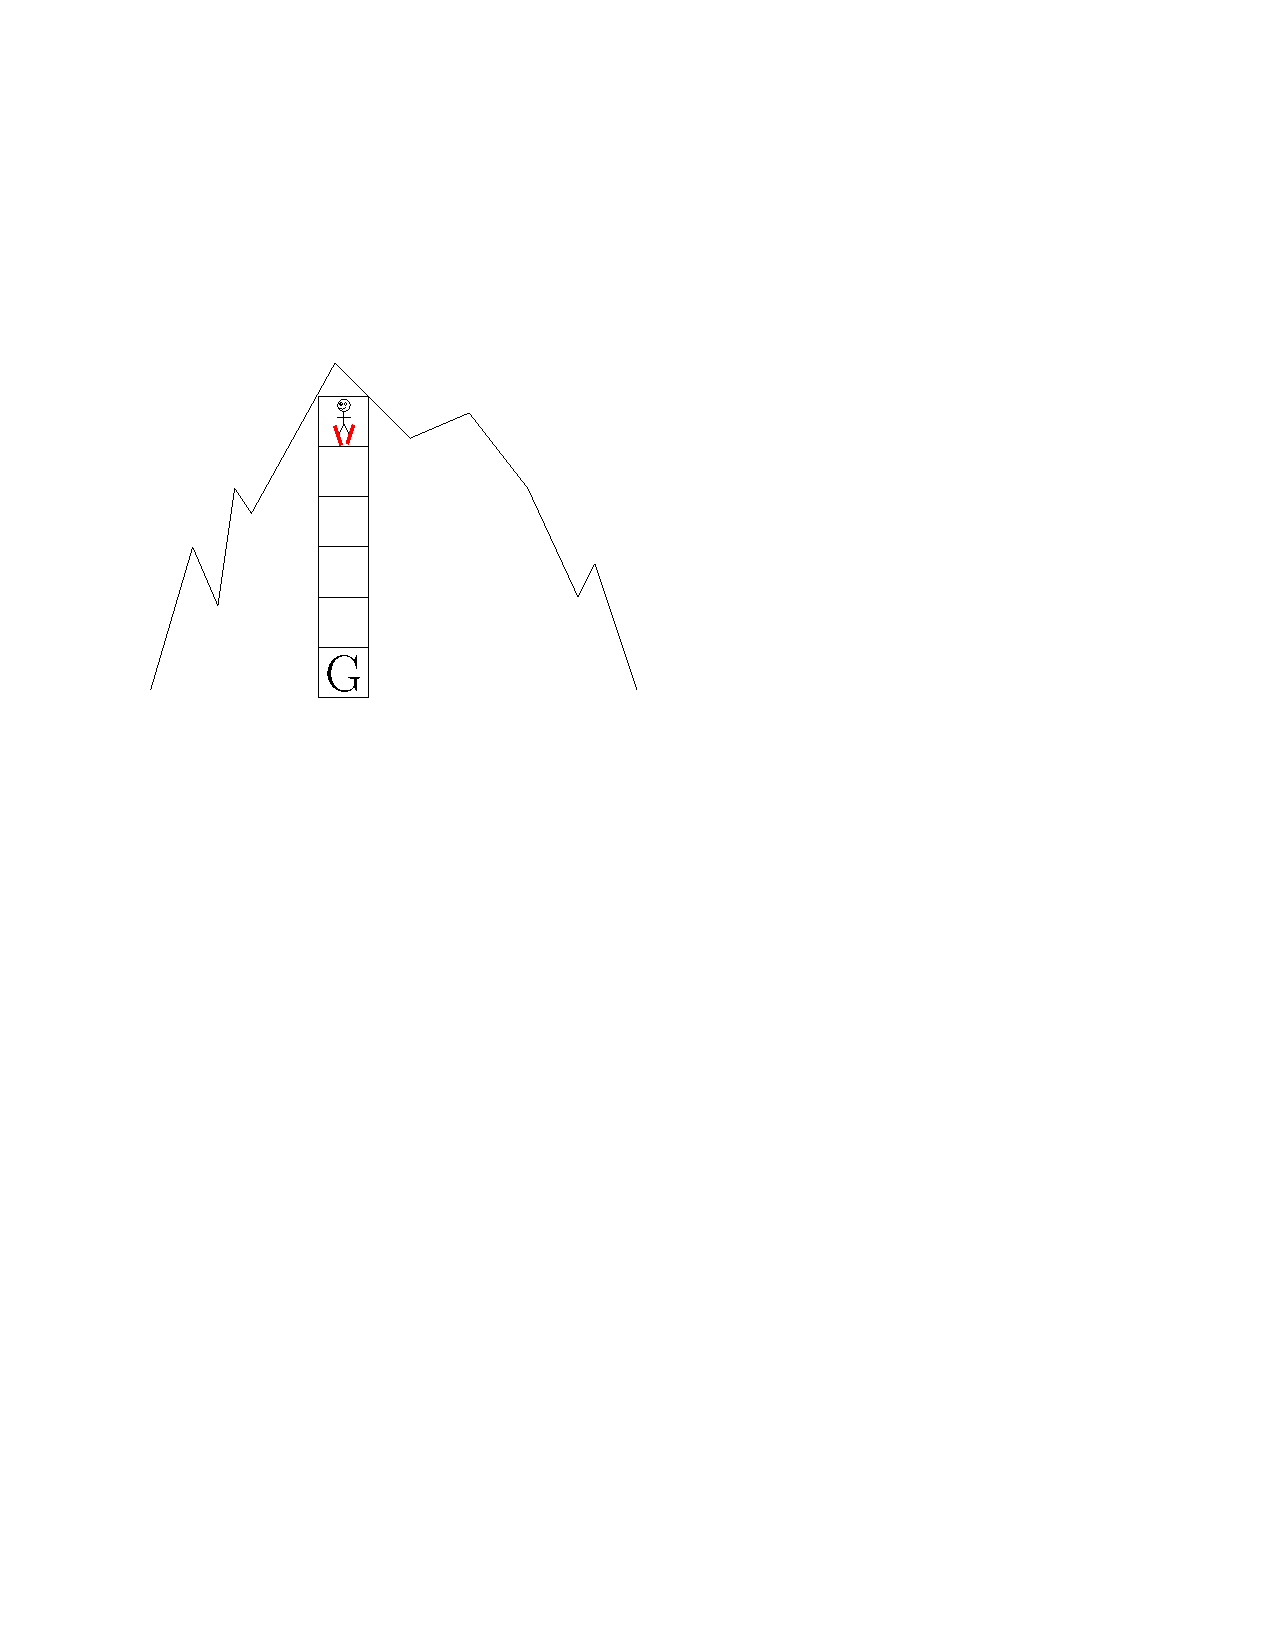
\includegraphics[width=0.5\textwidth]{hw1-skiing.pdf}

Consider the above figure.  If Alice's first action is ``accelerate''
then she will end up in the second square down with a velocity of
$1$.  If she then ``coasts'' then she will end up in the third square
down with a velocity of $1$.  If she ``accelerates'' again, she will
end up in the fifth square down with a velocity of $2$.

Alice's goal is to reach the chair lift (marked ``G'') with a velocity
of zero.  (No, Alice cannot have negative velocities).  She would like
to get there as quickly as possible.  However, if she has a non-zero
velocity at the goal, she skies into the parking lot and destroys her
skis.

% Ditto about commenting out the problem definition above.

\begin{enumerate}
\item If the mountain is $N$ units tall (eg., it is $N=6$ units tall in
the figure), what is the size of the state space?  Justify your
answer.  (You may ignore ``unreachable'' states.)  What are the
start/goal states?

\item Give an example of a state that is not reachable.  Suppose that
Alice cannot coast (she must either accelerate or decelerate): does this
yield \emph{more} unreachable states? If so, give an example of one and
justify your answer either way.

\item Is Alice's current elevation (i.e., distance from the chair lift)
an admissible heuristic?  Why or why not?

\item State and justify a non-trivial, admissible heuristic for this
problem which is \emph{not} current elevation.
\end{enumerate}

\end{document}
